\documentclass[12pt, a4paper]{article}

\usepackage[english]{babel}
\usepackage{lmodern}
\usepackage[utf8]{inputenc}
\usepackage[T1]{fontenc}
\usepackage[pdftex]{graphicx}
\usepackage{amsmath, amssymb}
\usepackage[hidelinks,unicode]{hyperref}
\usepackage{float}
\usepackage{listings}
\usepackage{tikz}
\usepackage{xcolor}
\usepackage{tabularx}
\usepackage[final]{pdfpages}
\usepackage{syntax}
\usepackage{caption}
\usepackage{subcaption}
\usepackage{amsfonts}
\usepackage{wrapfig}


\definecolor{mauve}{rgb}{0.58,0,0.82}
\usetikzlibrary{shapes,positioning,matrix,arrows}

\newcommand{\img}[1]{(viz obr. \ref{#1})}

\definecolor{pblue}{rgb}{0.13,0.13,1}
\definecolor{pgreen}{rgb}{0,0.5,0}
\definecolor{pred}{rgb}{0.9,0,0}
\definecolor{pgrey}{rgb}{0.46,0.45,0.48}


\lstdefinestyle{flex}{
    frame=tb,
    aboveskip=3mm,
    belowskip=3mm,
    showstringspaces=false,
    columns=flexible,
    basicstyle={\small\ttfamily},
    numbers=none,
    numberstyle=\tiny\color{black},
    keywordstyle=\color{black},
    commentstyle=\color{black},
    stringstyle=\color{black},
    breaklines=true,
    breakatwhitespace=true,
    tabsize=3
}

\lstset{
    frame=tb,
    language=Python,
    aboveskip=3mm,
    belowskip=3mm,
    showstringspaces=false,
    columns=flexible,
    basicstyle={\small\ttfamily},
    numbers=none,
    numberstyle=\tiny\color{gray},
    keywordstyle=\color{blue},
    commentstyle=\color{pgreen},
    stringstyle=\color{mauve},
    breaklines=true,
    breakatwhitespace=true,
    tabsize=3
}


\let\oldsection\section
\renewcommand\section{\clearpage\oldsection}

\begin{document}
	% this has to be placed here, after document has been created
	% \counterwithout{lstlisting}{chapter}
	\renewcommand{\lstlistingname}{Ukázka kódu}
	\renewcommand{\lstlistlistingname}{Seznam ukázek kódu}
    \begin{titlepage}

        \centering

        \vspace*{\baselineskip}
        \begin{figure}[H]
        \centering
        
\includegraphics[width=7cm]{img/fav-logo.jpg}
        \end{figure}

        \vspace*{1\baselineskip}

        \vspace{0.75\baselineskip}

        \vspace{0.5\baselineskip}
        {KIV/VSS Semester Project Assignment}

        {\LARGE\sc Benchmarking A Payment Terminal Managemenent Server \\}

        \vspace{4\baselineskip}

        \vspace{0.5\baselineskip}

        {\sc\Large Stanislav Král \\}
        \vspace{0.5\baselineskip}
        {A20N0091P}

        \vfill

        {\sc Západočeská univerzita v Plzni\\
        Fakulta aplikovaných věd}

    \end{titlepage}

    % TOC
    \tableofcontents
    \pagebreak

\section{Introduction}

\begin{wrapfigure}{r}{0.38\textwidth}
    \centering
    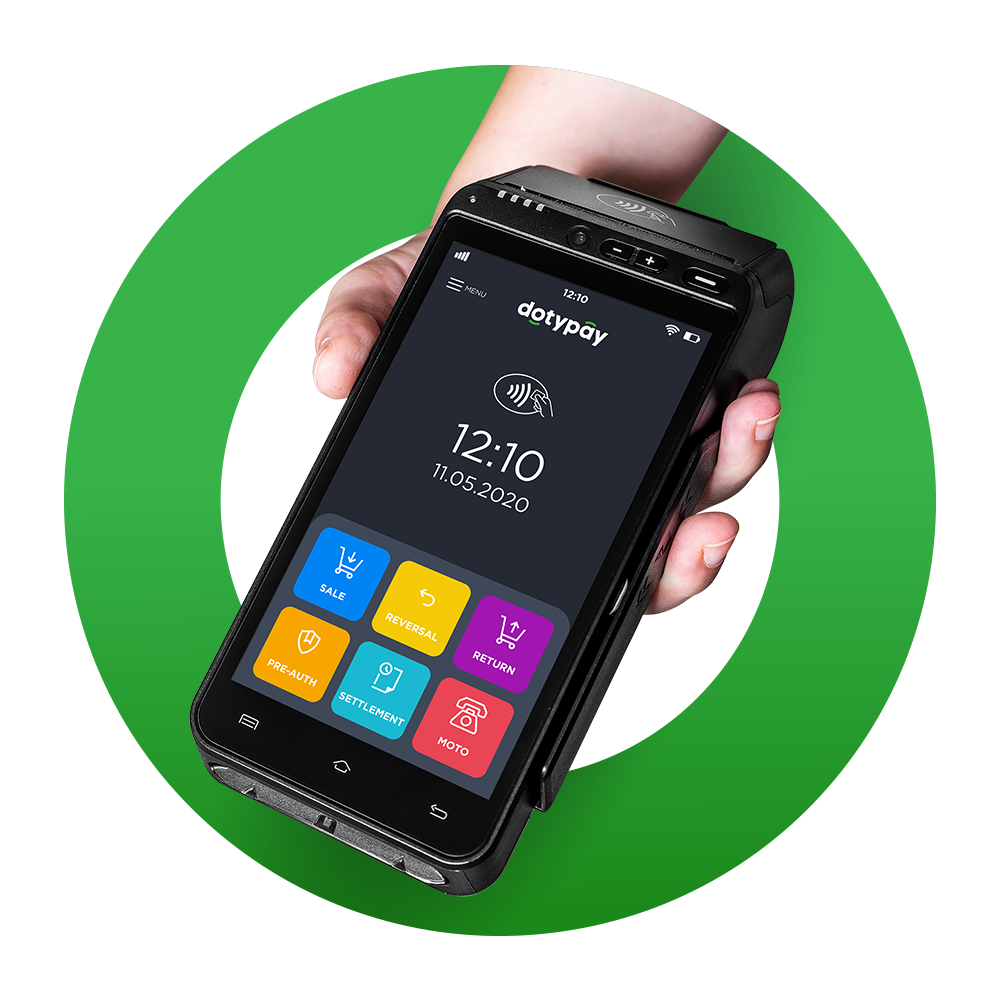
\includegraphics[width=.37\textwidth]{img/dotypay-payment-terminal.png}
    \captionof{figure}{Dotypay product landing page image}
\end{wrapfigure}

Dotypay\footnote{\url{https://dotypay.com/}} is a product that allows merchants to interface with payment cards to make electronic funds transfers via a payment terminal it offers.
The terminal is a mobile device running an Android OS with a built-in chip and contactless card reader with the support of magnetic stripe cards.
The fact that the terminal is running an Android OS means that it allows for utilization of various cash register applications that can be installed directly on the terminal. 
This reduces the number of devices the merchant has to operate in order to process customer orders to just a single all-in-one device.

The terminal comes with two preinstalled applications: Dotypay and Dotypay Launcher. The former is used for creating and processing payment, preauthorization and return transactations with the ability to preview the transaction and settlement history. The latter is used for device configuration which consists of following tasks:

\begin{itemize}
    \item \textbf{cryptographic keys setup} -- in order to securely process card payment transactions the terminal must be properly configured in the means of having all required cryptographic keys securely stored in the device storage,
    \item \textbf{merchant personalisation} -- configuration of the terminal based on the merchant it belongs to (currency code, country code,...),
    \item and \textbf{maintenance of the software installed} -- periodically check whether there are updates available to the installed software such as payment application, terminal firmware or cash register application.

\end{itemize}

Configuration and management of terminals happens on a dedicated web application, and is also accessible to merchants to view transaction history and analytics and other useful insights of made turn overs.

Dotypay also claims to charge smaller transaction fees than other payment processing products in the market.


\section{Dotypay Portal server}

As mentioned in the introduction Dotypay payment terminals have to retrieve their configuration from a remote server (Dotypay Portal) in order to be functioning properly. 
The Dotypay Portal server is the subject to be put under a test in order to investigate its capability to handle terminal requests.

The main component of the server is a Java application based on the Spring Boot framework that is dependent on following components:

\begin{itemize}
    \item \textbf{MS SQL database} -- main database used for persisting merchant data and terminal configuration,
    \item \textbf{Mongo database}  -- secondary database used to store transactions performed by terminals,
    \item \textbf{Amazon S3 storage}  -- object storage service for storing installation packages of terminal application as well as any merchant documents,
    \item \textbf{Amazon SQS} -- a queue service used for submitting transaction requests to the terminal,
    \item \textbf{SMTP server} -- a mail server for communication with merchants,
    \item and \textbf{Eddie TMS} -- a terminal management system by Monet+\footnote{Part of the EMV Payments service \url{https://www.monetplus.cz/emv-payments}}
\end{itemize}

It also dependent on other components such as online web application Rejstřík\footnote{\url{www.rejstrik.cz}}, MailChimp and OTRS.

\subsection{Hardware specification}
At the time of writing this document the Spring Boot application runs on an AWS node (2 vCPU and 4GB RAM plan), while the MS SQL database runs on another AWS node (2 vCPU and 2GB RAM plan).
Hardware configuration of other Amazon components is not known as they are supposed to be automatically scaled based on usage load as Amazon claims. The remaining components are not directly managed by Dotypay so their configuration is also not known. 

\subsection{Terminal synchronization with Dotypay Portal}
The Dotypay Launcher application that comes preinstalled on the payment terminals is responsible for periodically checking the Dotypay Portal server for terminal configuration. It does so by creating an HTTP request to the REST API interface of the server every 15 minutes with addition of a random delay up to 5 minutes.

During the processing of the synchronization request the server has to query the database for the terminal configuration. After querying the database the server responds with the configuration data. 

If the configuration contains any mandatory applications the terminal then proceeds to download installation packages from the server. The installation package data is fed to the terminal from the Amazon S3 storage.

In the past there has been a case where upon updating a version of a mandatory application in the Dotypay Portal a great number number of terminals after fetching the latest configuration started to download the application installation package at once. 
This load on the server resulted in its instability and increased response time as well as failed package downloads across most of the terminals. 

\subsection{Submission of a performed transaction}
Each transaction that is performed on the terminal is submitted to the server so that the history of transactions is preserved and can be viewed at later date elsewhere than in the terminal itself.
The transaction data is also used for creating insightful reports of merchant sales.

All transactions are submitted to the server even if they haven't been finished successfully (e.g. transaction declined by card scheme).

When the server receives a request to store an incoming transaction it performs only a minor processing and forwards the transaction to a MongoDB database instance, which is currently being implemented by a MongoDB Atlas service at Amazon.

The payment terminal is currently not capable of processing transactions when the connection to the Internet is not available, which means that a batch of multiple transactions coming from a single terminal to be stored in the database is not expected. 

As the number of merchants using the Dotypay product is continously increasing, the volume of transactions is following this trend.
Various spikes have been observed in the past in regards of the total transaction volume and count, however, no reports of service degradation have been reported so far.
For example, such spikes can be seen days before holidays, during lunch-time or after the usual time people finish their shift at work. During the rest of the day the usage of the server is somewhat evenly distributed, with the number of transactions slowly decreasing as night time comes by. In the early morning it eventually starts to increase again.


\end{document}

